% =====================================================================
% BMED365 (Spring 2027) — Lab 4: Differentiable Neurosymbolic AI Report
% Printable Companion Notebook Export: 02_instancenorm_trap_and_ltn_math.ipynb
% Compile with: pdflatex 02_instancenorm_trap_and_ltn_math_ipynb.tex (run twice)
% =====================================================================
\documentclass[10pt,a4paper]{article}

\usepackage[utf8]{inputenc}
\usepackage[T1]{fontenc}
\usepackage[english]{babel}
\usepackage{lmodern}
\usepackage{microtype}
\usepackage{graphicx}
\usepackage{booktabs}
\usepackage{xltabular}
\usepackage{tabularx}
\usepackage{array}
\usepackage[table]{xcolor}
\usepackage{amsmath,amssymb,mathtools}
\usepackage{enumitem}
\usepackage[margin=1.7cm,top=1.75cm,bottom=1.85cm,headheight=14pt]{geometry}
\usepackage{fancyhdr}
\usepackage{lastpage}
\usepackage{titlesec}
\usepackage[most]{tcolorbox}
\usepackage{listings}
\usepackage{float}
\usepackage{caption}
\usepackage[hyphens]{url}
\usepackage[
    colorlinks=true,
    linkcolor=uibblue,
    citecolor=uibblue,
    urlcolor=uibred,
    bookmarksnumbered=true,
    bookmarksopen=true,
    pdftitle={02_instancenorm_trap_and_ltn_math.ipynb -- InstanceNorm3d Coordinate-Erasure Trap and LTN Real-Logic Mathematics (BMED365 Spring 2027)},
    pdfauthor={Arvid Lundervold (University of Bergen & MMIV) -- BMED365 Spring 2027},
    pdfsubject={BMED365 Spring 2027 -- Differentiable Neurosymbolic AI Companion Notebook}
]{hyperref}
\def\UrlBreaks{\do\/\do-\do_\do.}
% Allow clean line breaks after underscores in long filenames & Python identifiers
\let\origunderscore\_
\renewcommand{\_}{\origunderscore\allowbreak}

% =====================================================================
% COLORS (UiB / MMIV / BMED365 House Style)
% =====================================================================
\definecolor{uibblue}{RGB}{0, 61, 115}
\definecolor{uibred}{RGB}{175, 28, 44}
\definecolor{kiwigreen}{RGB}{27, 138, 90}
\definecolor{amberwarn}{RGB}{165, 95, 0}
\definecolor{amberbg}{RGB}{255, 250, 240}
\definecolor{lightgray}{RGB}{246, 248, 250}
\definecolor{rowalt}{RGB}{243, 247, 252}
\definecolor{codebg}{RGB}{245, 248, 252}
\definecolor{codehdr}{RGB}{224, 234, 246}
\definecolor{outbg}{RGB}{250, 250, 250}
\definecolor{outhdr}{RGB}{236, 238, 240}
\definecolor{codekw}{RGB}{0, 75, 145}
\definecolor{codestr}{RGB}{155, 35, 45}
\definecolor{codecmt}{RGB}{90, 105, 118}

% =====================================================================
% TYPOGRAPHY, HEADERS & CALLOUT BOXES
% =====================================================================
\setlength{\parindent}{0pt}
\setlength{\parskip}{0.42em}
\setlength{\emergencystretch}{1.8em}
\setlist[itemize]{topsep=2pt,itemsep=2pt,leftmargin=1.45em}
\setlist[enumerate]{topsep=2pt,itemsep=2pt,leftmargin=1.65em}

\newcolumntype{L}[1]{>{\raggedright\arraybackslash}p{#1}}
\newcolumntype{C}[1]{>{\centering\arraybackslash}p{#1}}
\newcolumntype{R}[1]{>{\raggedleft\arraybackslash}p{#1}}
\newcolumntype{Y}{>{\raggedright\arraybackslash}X}

\titleformat{\section}{\large\bfseries\color{uibblue}}{\thesection}{0.65em}{}[\vspace{1pt}\color{uibblue!40}\titlerule]
\titleformat{\subsection}{\normalsize\bfseries\color{uibblue!88!black}}{\thesubsection}{0.55em}{}
\titleformat{\subsubsection}{\small\bfseries\color{uibblue!75!black}}{\thesubsubsection}{0.5em}{}
\titlespacing*{\section}{0pt}{1.05em}{0.4em}
\titlespacing*{\subsection}{0pt}{0.75em}{0.25em}
\titlespacing*{\subsubsection}{0pt}{0.55em}{0.2em}

\pagestyle{fancy}
\fancyhf{}
\fancyhead[L]{\footnotesize\textcolor{gray}{BMED365 (Spring 2027) $\cdot$ Neurosymbolic 7\,T MRI Package}}
\fancyhead[R]{\footnotesize\textcolor{gray}{\texttt{02\_instancenorm\_trap\_and\_ltn\_math.ipynb}}}
\fancyfoot[L]{\footnotesize\textcolor{gray}{University of Bergen \& MMIV $\cdot$ \href{https://github.com/arvidl/BMED365-2027}{\textcolor{gray}{github.com/arvidl/BMED365-2027}}}}
\fancyfoot[R]{\footnotesize\textcolor{gray}{Page \thepage{} of \pageref{LastPage}}}
\renewcommand{\headrulewidth}{0.4pt}
\renewcommand{\footrulewidth}{0.2pt}

\fancypagestyle{firstpage}{
    \fancyhf{}
    \fancyfoot[L]{\footnotesize\textcolor{gray}{University of Bergen \& MMIV $\cdot$ \href{https://github.com/arvidl/BMED365-2027}{\textcolor{gray}{github.com/arvidl/BMED365-2027}}}}
    \fancyfoot[R]{\footnotesize\textcolor{gray}{Page \thepage{} of \pageref{LastPage}}}
    \renewcommand{\headrulewidth}{0pt}
    \renewcommand{\footrulewidth}{0.2pt}
}

% --- Notebook Cell & Pedagogical Boxes ---
\newtcolorbox{seqbox}[1][]{
    enhanced, breakable,
    colback=lightgray, colframe=uibblue,
    colbacktitle=uibblue, coltitle=white,
    fonttitle=\bfseries\small, title={#1},
    boxrule=0.6pt, arc=2.5pt, left=7pt, right=7pt, top=5pt, bottom=5pt
}

\newtcolorbox{codebox}[1][]{
    enhanced, breakable,
    colback=codebg, colframe=uibblue!35,
    colbacktitle=codehdr, coltitle=uibblue!90!black,
    fonttitle=\ttfamily\scriptsize\bfseries, title={#1},
    boxrule=0.55pt, arc=2.2pt, left=6pt, right=6pt, top=3pt, bottom=3pt,
    toptitle=2.5pt, bottomtitle=2.5pt
}

\newtcolorbox{outbox}[1][]{
    enhanced, breakable,
    colback=outbg, colframe=gray!45,
    colbacktitle=outhdr, coltitle=black!75,
    fonttitle=\ttfamily\scriptsize\bfseries, title={#1},
    boxrule=0.5pt, arc=2.2pt, left=6pt, right=6pt, top=3pt, bottom=3pt,
    toptitle=2pt, bottomtitle=2pt
}

\newtcolorbox{clinbox}[1][]{
    enhanced, breakable,
    colback=amberbg, colframe=amberwarn,
    colbacktitle=amberwarn, coltitle=white,
    fonttitle=\bfseries\small, title={#1},
    boxrule=0.6pt, arc=2.5pt, left=7pt, right=7pt, top=5pt, bottom=5pt
}

\newtcolorbox{guidehdr}[1][]{
    enhanced,
    colback=kiwigreen!6, colframe=kiwigreen!75!black,
    borderline west={2.5pt}{0pt}{kiwigreen!85!black},
    boxrule=0.45pt, arc=2pt, left=7pt, right=7pt, top=3.5pt, bottom=3.5pt,
    before skip=0.7em, after skip=0.35em
}

% --- Listings Styles (UTF-8 literate support for pdflatex) ---
\lstdefinestyle{pybmed}{
    language=Python,
    basicstyle=\ttfamily\scriptsize,
    keywordstyle=\bfseries\color{codekw},
    stringstyle=\color{codestr},
    commentstyle=\itshape\color{codecmt},
    showstringspaces=false,
    breaklines=true,
    breakatwhitespace=false,
    breakindent=12pt,
    columns=fullflexible,
    keepspaces=true,
    upquote=true,
    aboveskip=2pt,
    belowskip=2pt,
    xleftmargin=0pt,
    xrightmargin=0pt,
    literate={±}{{$\pm$}}1
             {³}{{\textsuperscript{3}}}1
             {×}{{$\times$}}1
             {é}{{\'e}}1
             {ö}{{\"o}}1
             {Ł}{{\L{}}}1
             {Δ}{{$\Delta$}}1
             {α}{{$\alpha$}}1
             {–}{{--}}1
             {—}{{---}}1
             {≥}{{$\ge$}}1
             {≤}{{$\le$}}1
             {⊂}{{$\subset$}}1
             {∈}{{$\in$}}1
             {→}{{$\to$}}1
             {…}{{\ldots}}1
}

\lstdefinestyle{bashbmed}{
    language=bash,
    basicstyle=\ttfamily\scriptsize,
    keywordstyle=\bfseries\color{codekw},
    stringstyle=\color{codestr},
    commentstyle=\itshape\color{codecmt},
    showstringspaces=false,
    breaklines=true,
    breakatwhitespace=false,
    breakindent=12pt,
    columns=fullflexible,
    keepspaces=true,
    upquote=true,
    aboveskip=2pt,
    belowskip=2pt,
    xleftmargin=0pt,
    xrightmargin=0pt
}

\lstdefinestyle{outbmed}{
    basicstyle=\ttfamily\scriptsize\color{black!85},
    showstringspaces=false,
    breaklines=true,
    breakatwhitespace=false,
    columns=fullflexible,
    keepspaces=true,
    upquote=true,
    aboveskip=1pt,
    belowskip=1pt,
    xleftmargin=0pt,
    xrightmargin=0pt
}

\lstdefinestyle{outbmedwide}{
    basicstyle=\ttfamily\fontsize{6.3pt}{7.6pt}\selectfont\color{black!85},
    showstringspaces=false,
    breaklines=true,
    breakatwhitespace=false,
    columns=fullflexible,
    keepspaces=true,
    upquote=true,
    aboveskip=1pt,
    belowskip=1pt,
    xleftmargin=0pt,
    xrightmargin=0pt
}

\newcommand{\ghblob}{https://github.com/arvidl/BMED365-2027/blob/main}
\newcommand{\colabbase}{https://colab.research.google.com/github/arvidl/BMED365-2027/blob/main}
\newcommand{\repodir}{Lab4-Comp-Imag/Kiwi-challenge/docs/neurosymbolic-report}
\newcommand{\colabbtn}[1]{%
  \href{#1}{\tcbox[on line, arc=2.5pt, boxsep=0pt, left=6pt, right=6pt, top=2.5pt, bottom=2.5pt,
    colback=amberwarn!85!yellow, colframe=white!70!amberwarn, boxrule=0.5pt]{%
    \sffamily\bfseries\scriptsize\color{white}Open in Google Colab}}%
}

% =====================================================================
\begin{document}
\thispagestyle{firstpage}

% --- TITLE BANNER ---
\begin{tcolorbox}[
    enhanced, colback=uibblue, colframe=uibblue,
    arc=3.5pt, left=12pt, right=12pt, top=9pt, bottom=9pt
]
{\Large\bfseries\color{white} Companion Notebook 02 --- The \texttt{InstanceNorm3d} Coordinate-Erasure Trap \& LTN Real-Logic Math\\[2pt]
{\large Affine-Invariance Proof, Bayes Log-Odds \texttt{Organ-GPS}, Fuzzy $T$-Norms \& $p$-Mean Autograd Verification}}\\[4pt]
{\normalsize\color{white!90} BMED365 --- Computational Imaging, Modeling and AI in Biomedicine (Spring 2027)}\\[3pt]
{\footnotesize\color{white!84}
Arvid Lundervold (University of Bergen \& MMIV) $\;\cdot\;$ Reproduces Report Sec.\ 2.3--2.4, 3.2, Figs.\ 4--5, Table~4 \& Appendices~B, D $\;\cdot\;$ Measured runtime: \texttt{7.2 s} (MPS)
}\\[6pt]
\colabbtn{\colabbase/\repodir/notebooks/02_instancenorm_trap_and_ltn_math.ipynb}\hspace{8pt}
{\footnotesize\href{\ghblob/\repodir/notebooks/02_instancenorm_trap_and_ltn_math.ipynb}{\textcolor{white}{\underline{\texttt{02\_instancenorm\_trap\_and\_ltn\_math.ipynb} on GitHub}}}}\hspace{10pt}
{\footnotesize\href{\ghblob/\repodir/neurosymbolic-kiwi-report.pdf}{\textcolor{white}{\underline{Technical Report PDF}}}}
\end{tcolorbox}

\begin{seqbox}[Neurosymbolic 7\,T MRI Technical Report --- Companion Package (\texttt{docs/neurosymbolic-report})]
{\footnotesize Companion to \href{\ghblob/\repodir/neurosymbolic-kiwi-report.pdf}{\textbf{\texttt{neurosymbolic-kiwi-report.pdf}}} and shared library \href{\ghblob/\repodir/notebooks/kiwi_ns_lib.py}{\texttt{kiwi\_ns\_lib.py}} (\href{\ghblob/\repodir/notebooks/kiwi_ns_lib_py.pdf}{\textit{annotated PDF}}):}
\begin{enumerate}[start=1, itemsep=1.2pt, topsep=2pt, font=\footnotesize]
    \item \href{\ghblob/\repodir/notebooks/01_data_geometry_and_prior_audit.ipynb}{\texttt{01\_data\_geometry\_and\_prior\_audit.ipynb}} --- 7\,T MRI geometry, empirical audit of Priors 1--3, tri-planar Micro-GT superimposition \& manual GT editing guide (Figs.\ 1--3, Table~3; 27.4\,s MPS).
    \item \textbf{\texttt{02\_instancenorm\_trap\_and\_ltn\_math.ipynb} (this notebook)} --- Experimental proof of \texttt{InstanceNorm3d} coordinate erasure, Bayes Log-Odds \texttt{Organ-GPS}, fuzzy $T$-norms \& LTN $p$-mean autograd sweep (Figs.\ 4--5, Table~4; 7.2\,s MPS).
    \item \href{\ghblob/\repodir/notebooks/03_multiseed_ablation_and_calibration.ipynb}{\texttt{03\_multiseed\_ablation\_and\_calibration.ipynb}} --- 3-seed $\times$ 6-model controlled ablation, operating-point calibration shift \& unmasked whole-organ OOD safety (Figs.\ 6--7, Tables~5--6; 555.1\,s MPS).
    \item \href{\ghblob/\repodir/notebooks/04_mechanistic_interpretability_and_biomarkers.ipynb}{\texttt{04\_mechanistic\_interpretability\_and\_biomarkers.ipynb}} --- Causal neural--symbolic division of labor ($z_{\text{GPS}}$), Mat\'ern hard-core split sweep, error anatomy \& 128-slice NIfTI biomarkers (Figs.\ 8--9, Tables~7--8; 99.3\,s MPS).
    \item \href{\ghblob/\repodir/notebooks/05_axiom_stress_tests_and_clinical_translation.ipynb}{\texttt{05\_axiom\_stress\_tests\_and\_clinical\_translation.ipynb}} --- Pathological mass-effect center-shift ($\Delta r \in [0, 8]$\,mm) \& radial-scale ($\alpha \in [0.80, 1.25]$) stress tests vs.\ rigid post-hoc masks (Fig.\ 10, Table~9; 55.4\,s MPS).
\end{enumerate}
\end{seqbox}

\subsection*{Purpose}
\begin{enumerate}
\item Prove experimentally on real equatorial (\texttt{z = 56..71}), mid-latitude (\texttt{z = 32..47}), and polar (\texttt{z = 0..15}) crops that patch-wise \texttt{nn.InstanceNorm3d} completely erases absolute organ location --- motivating our \textbf{Bayes Log-Odds \texttt{Organ-GPS}} architecture (\texttt{+353} parameters).
\item Compare three classical fuzzy implication families (\textbf{Product /\allowbreak{} Reichenbach}, \textbf{\L{}ukasiewicz}, \textbf{G\"odel}) on gradient smoothness and dead zones.
\item Compute the exact loss and gradient amplification of LTN's generalized $p$-mean universal quantifier across $p \in [1, 8]$ on a simulated \texttt{40,960}-voxel polar cube containing \texttt{0.8\%} (\texttt{328} voxels) vascular false positives.
\end{enumerate}

\section*{0. Environment Setup: Portable Execution, Shared Library \& Autograd Engine}
\addcontentsline{toc}{section}{\texorpdfstring{0. Environment Setup: Portable Execution, Shared Library \& Autograd Engine}{0. Environment Setup: Portable Execution, Shared Library and Autograd Engine}}

\begin{guidehdr}
{\small\bfseries\color{kiwigreen!75!black}Conceptual \& Practical Motivation}
\end{guidehdr}
Before running any mathematical proof or numerical experiment, we configure a reproducible runtime that works identically whether you run locally (macOS Apple Silicon or Linux/\allowbreak{}CUDA) or click \textbf{Open in Colab}:

\begin{itemize}
\item \textbf{Zero-drift shared library (\texttt{kiwi\_ns\_lib.py}):} Rather than copy-pasting coordinate transforms, 3D U-Net architectures, and fuzzy-logic operators across five separate notebooks---where small edits could silently drift out of sync with the technical report---all notebooks import the same module \texttt{kiwi\_ns\_lib.py} (automatically downloaded from GitHub \texttt{main} in standalone Colab sessions).
\item \textbf{Scientific imaging \& analysis stack:} \texttt{nibabel}, \texttt{scipy}, and \texttt{skimage} read the 3D 7\,T RARE MRI volume (spacing $s = (0.2344,\, 0.2344,\, 0.5000)\,\text{mm}$) and construct anatomical organ coordinates; \texttt{numpy}, \texttt{pandas}, and \texttt{matplotlib} tabulate metrics and render report-ready figures.
\item \textbf{PyTorch (\texttt{torch}) as both a neural layer and a calculus engine:} We use PyTorch for two distinct mathematical jobs in this notebook:
\begin{enumerate}
\item Executing the exact 3D normalization operator \texttt{nn.InstanceNorm3d} and counting exact parameter budgets across our three 3D network families.
\item Computing exact partial derivatives $\partial \mathcal{L}_p / \partial v_i$ via \textbf{reverse-mode automatic differentiation (autograd)} so we can verify our analytical LTN quantifier gradients directly in \texttt{float32} arithmetic (note that \texttt{float32} machine precision is $\approx 1.19 \times 10^{-7}$, which explains the $\sim 5 \times 10^{-7}$ residual noise floor we will observe in Section 1).
\end{enumerate}
\item \textbf{Portable device \& output resolution:} \texttt{kns.get\_best\_device()} selects the fastest available backend at runtime (\texttt{CUDA} $\to$ Apple \texttt{MPS} $\to$ \texttt{CPU}), and \texttt{kns.resolve\_report\_dirs()} resolves \texttt{FIG\_DIR} and \texttt{RES\_DIR} for saving Figures 3--4 and \texttt{nb02\_instancenorm\_and\_ltn.json}.
\end{itemize}

\begin{codebox}[{In [1] $\cdot$ Python --- Environment setup, \texttt{kiwi\_ns\_lib.py} bootstrap \& autograd engine}]
\begin{lstlisting}[style=pybmed]
import json
import sys
import urllib.request
from pathlib import Path

# Auto-fetch shared library `kiwi_ns_lib.py` if opened standalone in Google Colab
if not Path("kiwi_ns_lib.py").exists():
    for cand in [Path("docs/neurosymbolic-report/notebooks/kiwi_ns_lib.py"),
                 Path("Lab4-Comp-Imag/Kiwi-challenge/docs/neurosymbolic-report/notebooks/kiwi_ns_lib.py")]:
        if cand.exists():
            sys.path.insert(0, str(cand.parent.resolve()))
            break
    else:
        url = "https://raw.githubusercontent.com/arvidl/BMED365-2027/main/Lab4-Comp-Imag/Kiwi-challenge/docs/neurosymbolic-report/notebooks/kiwi_ns_lib.py"
        print("Downloading kiwi_ns_lib.py from GitHub main for Colab session...")
        urllib.request.urlretrieve(url, "kiwi_ns_lib.py")

if str(Path.cwd()) not in sys.path:
    sys.path.insert(0, str(Path.cwd()))

import importlib.util
for pkg in ("nibabel", "torch"):
    if importlib.util.find_spec(pkg) is None:
        import subprocess
        subprocess.check_call([sys.executable, "-m", "pip", "install", "-q", pkg])

get_ipython().run_line_magic("matplotlib", "inline")
import matplotlib.pyplot as plt
import numpy as np
import pandas as pd
import torch
from scipy import ndimage as ndi
from scipy.spatial.distance import cdist
from skimage import measure

plt.rcParams.update({"figure.dpi": 130, "savefig.dpi": 200, "font.size": 9.5})

import kiwi_ns_lib as kns

DEVICE = kns.get_best_device()
FIG_DIR, RES_DIR = kns.resolve_report_dirs()
print(f"Device: {DEVICE} | Figures -> {FIG_DIR} | Results -> {RES_DIR}")
\end{lstlisting}
\end{codebox}
\begin{outbox}[{Out [1] $\cdot$ stdout}]
\begin{lstlisting}[style=outbmed]
Device: mps | Figures -> <BMED365-2027>/Lab4-Comp-Imag/Kiwi-challenge/docs/neurosymbolic-report/figures | Results -> <BMED365-2027>/Lab4-Comp-Imag/Kiwi-challenge/docs/neurosymbolic-report/results
\end{lstlisting}
\end{outbox}

\section*{1. Direct Proof of \texttt{InstanceNorm3d} Coordinate Erasure Across Three Anatomical Latitudes}
\addcontentsline{toc}{section}{\texorpdfstring{1. Direct Proof of \texttt{InstanceNorm3d} Coordinate Erasure Across Three Anatomical Latitudes}{1. Direct Proof of InstanceNorm3d Coordinate Erasure Across Three Anatomical Latitudes}}

\begin{guidehdr}
{\small\bfseries\color{kiwigreen!75!black}Conceptual \& Mathematical Guide: The Coordinate-Erasure Trap \& Bayes Log-Odds \texttt{Organ-GPS}}
\end{guidehdr}

\subsubsection*{1.1 Biomedical Motivation: Why a Local 3D U-Net Needs Global Organ Coordinates}
A standard 3D convolutional network slides the same $3 \times 3 \times 3$ filters over every voxel (\textbf{translation equivariance}). That property is great for sample efficiency---a seed detector learned on one side of the equatorial ring works on the opposite side---but creates a dangerous blind spot in 3D anatomy: a dark fibrous vascular bundle at the woody polar cap (\texttt{z = 0..15}, where \textbf{zero} seeds exist) looks locally almost identical to a dark seed in the equatorial inner pericarp (\texttt{z = 56..71}).

To provide global anatomical context, \texttt{kns.make\_3ch\_and\_gps()} builds a 3-channel dimensionless \textbf{Organ-GPS} coordinate field $\mathbf{c}(\mathbf{x})$ at every voxel $\mathbf{x} = (x, y, z)$:
\[
\mathbf{c}(\mathbf{x}) = \Bigl(\,\tilde{r}(\mathbf{x}),\;\; \bigl(\tilde{r}(\mathbf{x}) - 0.43\bigr)^2,\;\; \tilde{p}_z(\mathbf{x})\,\Bigr),
\]
where:
\begin{itemize}
\item $\tilde{r}(\mathbf{x}) = \operatorname{clip}\!\left(\frac{\sqrt{(x - c_x(z))^2 + (y - c_y(z))^2}}{R_{\text{fruit}}(z)},\, 0,\, 1.5\right)$ is the slice-normalized radial depth ($0$ at the central columella axis, $1$ at the outer skin; real seeds reside inside the inner pericarp $\tilde{r} \in [0.22, 0.65]$);
\item $(\tilde{r}(\mathbf{x}) - 0.43)^2$ measures symmetric quadratic distance from the mid-pericarp ring center ($\tilde{r} = 0.43$);
\item $\tilde{p}_z(\mathbf{x}) = \left|\frac{2z}{Z - 1} - 1\right| \in [0, 1]$ (with $Z = 128$ axial slices) is the \textbf{normalized pole distance} ($0$ at the equator $z \approx 63.5$, rising linearly to $1$ at the woody poles $z = 0$ and $z = 127$).
\end{itemize}

\subsubsection*{1.2 Mathematical Proof: Why \texttt{InstanceNorm3d} Erases Global Coordinates}
In 3D medical imaging, GPU memory forces tiny batch sizes ($B = 1$--$4$), making \texttt{BatchNorm3d} noisy. Consequently, modern medical CNNs (such as \texttt{nnU-Net}) default to \textbf{3D Instance Normalization (\texttt{nn.InstanceNorm3d})}, which standardizes \textit{each 3D patch $b$ and each channel $c$ independently} across its patch voxels $\Omega_P$:
\[
\operatorname{IN}(u)_{b,c}(\mathbf{x}) = \gamma_c\,\frac{u_{b,c}(\mathbf{x}) - \mu_{b,c}}{\sqrt{\sigma_{b,c}^2 + \epsilon}} + \beta_c,
\]
where $\mu_{b,c} = \frac{1}{|\Omega_P|}\sum_{\mathbf{x} \in \Omega_P} u_{b,c}(\mathbf{x})$, $\sigma_{b,c}^2 = \frac{1}{|\Omega_P|}\sum_{\mathbf{x} \in \Omega_P} \bigl(u_{b,c}(\mathbf{x}) - \mu_{b,c}\bigr)^2$, and $\epsilon = 10^{-5}$. (The code cell uses \texttt{affine=False}, i.e., $\gamma_c = 1, \beta_c = 0$; even with learnable \texttt{affine=True}, the same global $\gamma_c, \beta_c$ apply to every patch and cannot restore erased patch-specific location offsets.)

\textbf{Affine-Invariance (Coordinate-Erasure) Theorem:} Suppose two patches have coordinate fields related by any positive scale $a > 0$ and constant shift $b \in \mathbb{R}$, so $u_2(\mathbf{x}) = a\,u_1(\mathbf{x}) + b$ for all $\mathbf{x} \in \Omega_P$. Because $\mu(u_2) = a\,\mu(u_1) + b$ and $\sigma(u_2) = a\,\sigma(u_1)$, both $a$ and $b$ cancel algebraically (as $\epsilon \to 0$):
\[
\operatorname{IN}(u_2)(\mathbf{x}) = \frac{\bigl(a\,u_1(\mathbf{x}) + b\bigr) - \bigl(a\,\mu(u_1) + b\bigr)}{a\,\sigma(u_1)} = \frac{u_1(\mathbf{x}) - \mu(u_1)}{\sigma(u_1)} = \operatorname{IN}(u_1)(\mathbf{x}).
\]

Watch how this theorem plays out across the three real 16-slice crops extracted below:
\begin{itemize}
\item \textbf{Mid-Latitude (\texttt{z = 32..47}) vs. Polar Cap (\texttt{z = 0..15}):} Both crops lie strictly on the same side of the equator ($z < 63.5$), so $\tilde{p}_z(z) = 1 - \frac{2z}{127}$ is a pure linear ramp with identical slope $-\frac{2}{127}$ per slice and a constant vertical offset $b = \frac{64}{127} \approx +0.504$ ($a = 1$). After \texttt{InstanceNorm3d}, the entire latitude gap vanishes---both curves collapse onto a \textbf{bit-identical} diagonal line (max pointwise difference $\sim 5 \times 10^{-7}$, pure \texttt{float32} rounding + $\epsilon$). Even a preceding $3 \times 3 \times 3$ convolution preserves linearity on a linear ramp, so naive \texttt{CoordConv3D} cannot escape this trap!
\item \textbf{Equator (\texttt{z = 56..71}):} Because this crop straddles $z = 63.5$, $|2z/127 - 1|$ bends into a shallow V-shape; \texttt{InstanceNorm3d} still collapses its mean to \texttt{0.000000} and stretches its tiny variation to unit variance.
\end{itemize}

\subsubsection*{1.3 The Architectural Fix: Un-Normalized Bayes Log-Odds \texttt{Organ-GPS} (\texttt{+353} Parameters)}
Rather than feeding $\mathbf{c}(\mathbf{x})$ through \texttt{InstanceNorm3d}, \textbf{\texttt{AdditiveBayesOrganNet3D}} isolates the raw physical coordinates in a tiny \textbf{un-normalized} 2-layer $1 \times 1 \times 1$ MLP ($3 \to 16 \to 16 \to 1$ with \texttt{SiLU}), adding only $(3{\times}16 + 16) + (16{\times}16 + 16) + (16{\times}1 + 1) = \mathbf{353}$ parameters ($+0.10\%$ over the 340,450-parameter baseline). Assuming conditional independence of local MRI appearance $\mathbf{X}_3$ and global position $\mathbf{c}$ given seed class $Y \in \{0, 1\}$, Bayes' theorem factorizes posterior odds into a local likelihood ratio times an anatomical spatial prior:
\[
\frac{P(Y = 1 \mid \mathbf{X}_3, \mathbf{c})}{P(Y = 0 \mid \mathbf{X}_3, \mathbf{c})} = \underbrace{\frac{P(\mathbf{X}_3 \mid Y = 1)}{P(\mathbf{X}_3 \mid Y = 0)}}_{\text{Local appearance likelihood ratio}} \times \underbrace{\frac{P(Y = 1 \mid \mathbf{c})}{P(Y = 0 \mid \mathbf{c})}}_{\text{Anatomical spatial prior odds}}.
\]
Taking the natural logarithm converts multiplication of odds into \textbf{exact addition of logits (log-odds)}:
\[
z_{\text{total}}(\mathbf{x}) = \underbrace{z_{\text{app}}\bigl(\mathbf{f}_\theta(\mathbf{X}_3)\bigr)}_{\text{3D U-Net appearance head}} + \underbrace{z_{\text{GPS}}\bigl(\mathbf{c}(\mathbf{x});\, \psi\bigr)}_{\text{Un-normalized Organ-GPS (+353 params)}}, \qquad p_\theta(\mathbf{x}) = \sigma\bigl(z_{\text{total}}(\mathbf{x})\bigr).
\]
We also count \textbf{\texttt{CoupledOrganNet3D}} (\texttt{+864} params), which concatenates the un-normalized 16-channel GPS embedding with U-Net decoder features for nonlinear interaction.

\subsubsection*{1.4 What the Code Below Computes (Figure 3)}
\begin{enumerate}
\item Loads the 7\,T kiwifruit MRI (\texttt{ds}) and crops three real $64 \times 40 \times 16$ patches (\texttt{gps\_eq}, \texttt{gps\_mid}, \texttt{gps\_pol}).
\item Applies \texttt{nn.InstanceNorm3d(3, affine=False)} and compares channel 2 ($\tilde{p}_z$) along the patch center line before and after normalization, printing the patch means and maximum pointwise difference.
\item Audits exact parameter counts for \texttt{MultiTaskUNet3D}, \texttt{AdditiveBayesOrganNet3D}, and \texttt{CoupledOrganNet3D}.
\item Renders \textbf{Figure 3}: \textbf{(a)} raw separated latitudes, \textbf{(b)} bit-identical collapse of Mid-Lat and Pole under \texttt{InstanceNorm3d}, and \textbf{(c)} the preserved inside-fruit radial distributions $\tilde{r} = r / R_{\text{fruit}}$ seen by un-normalized \texttt{Organ-GPS} (an equatorial crop covers interior tissue $\tilde{r} \le 0.72$, whereas an equal-sized polar crop spans out to the skin $\tilde{r} \approx 1.0$).
\end{enumerate}

\begin{codebox}[{In [2] $\cdot$ Python --- Experimental proof of \texttt{InstanceNorm3d} coordinate erasure \& parameter audit}]
\begin{lstlisting}[style=pybmed]
ds = kns.load_kiwi_dataset()

# Extract three 64x40x16 crops spanning Equator, Mid-Latitude, and Polar Cap
_, gps_eq  = kns.make_3ch_and_gps(ds, 128, 192, 128, 168, 56, 72)
_, gps_mid = kns.make_3ch_and_gps(ds, 112, 176, 112, 152, 32, 48)
_, gps_pol = kns.make_3ch_and_gps(ds, 96,  160, 96,  136, 0,  16)

inorm = torch.nn.InstanceNorm3d(3, affine=False)
g_eq_in, g_mid_in, g_pol_in = inorm(gps_eq), inorm(gps_mid), inorm(gps_pol)

z_eq_r, z_mid_r, z_pol_r = [g[0, 2, 32, 20, :].numpy() for g in (gps_eq, gps_mid, gps_pol)]
z_eq_i, z_mid_i, z_pol_i = [g[0, 2, 32, 20, :].numpy() for g in (g_eq_in, g_mid_in, g_pol_in)]

max_diff_mid_pol_after = float(np.max(np.abs(z_mid_i - z_pol_i)))
print(f"RAW pole means         -> Equator={z_eq_r.mean():.3f} | Mid-Lat={z_mid_r.mean():.3f} | Pole={z_pol_r.mean():.3f}")
print(f"AFTER InstanceNorm3d   -> Equator={z_eq_i.mean():.6f} | Mid-Lat={z_mid_i.mean():.6f} | Pole={z_pol_i.mean():.6f}")
print(f"Max pointwise diff between Mid-Latitude (z=32..47) and Polar Cap (z=0..15) AFTER InstanceNorm3d: {max_diff_mid_pol_after:.2e} (IDENTICAL!)")

# Parameter counts of all three model families
n_base = sum(p.numel() for p in kns.MultiTaskUNet3D(3).parameters())
n_add = sum(p.numel() for p in kns.AdditiveBayesOrganNet3D().parameters())
n_cpl = sum(p.numel() for p in kns.CoupledOrganNet3D().parameters())
print(f"Params -> MultiTaskUNet3D: {n_base:,} | AdditiveBayesOrganNet3D: {n_add:,} (+{n_add-n_base}) | CoupledOrganNet3D: {n_cpl:,} (+{n_cpl-n_base})")

# Figure 3: 3-Panel Coordinate-Erasure Proof
fig, axes = plt.subplots(1, 3, figsize=(15.6, 3.85))
s_idx = np.arange(16)

axes[0].plot(s_idx, z_eq_r,  "o-", color="#1b8a5a", lw=2.0, label="Equator (z=56..71)")
axes[0].plot(s_idx, z_mid_r, "^-", color="#2980b9", lw=2.0, label="Mid-Latitude (z=32..47)")
axes[0].plot(s_idx, z_pol_r, "s-", color="#d95f02", lw=2.0, label="Polar Cap (z=0..15)")
axes[0].set_ylim(-0.06, 1.08)
axes[0].set_xlabel("Local Slice Offset Within 16-Slice Patch")
axes[0].set_ylabel("Raw Pole Distance |2z/Z - 1|")
axes[0].set_title("(a) True Metric Organ-GPS Input\nThree latitudes cleanly separated")
axes[0].legend(fontsize=7.8)
axes[0].grid(alpha=0.25)

axes[1].plot(s_idx, z_eq_i,  "o-", color="#1b8a5a", lw=2.0, label="Equator after InstanceNorm3d")
axes[1].plot(s_idx, z_mid_i, "^-", color="#2980b9", lw=2.6, label="Mid-Lat after InstanceNorm3d")
axes[1].plot(s_idx, z_pol_i, "s--", color="#d95f02", lw=1.8, markersize=4.5, label="Pole after InstanceNorm3d")
axes[1].set_xlabel("Local Slice Offset Within 16-Slice Patch")
axes[1].set_ylabel("Standardized Channel Value")
axes[1].set_title("(b) After InstanceNorm3d (Naive CoordConv)\nMid-Lat & Pole become BIT-IDENTICAL!")
axes[1].legend(fontsize=7.6)
axes[1].grid(alpha=0.25)

m_eq = ds.fruit_mask[128:192, 128:168, 56:72]
m_pol = ds.fruit_mask[96:160, 96:136, 0:16]
axes[2].hist(gps_eq[0, 0].numpy()[m_eq], bins=24, alpha=0.58, color="#1b8a5a", density=True, label="Inside-fruit r/R (Equator)")
axes[2].hist(gps_pol[0, 0].numpy()[m_pol], bins=24, alpha=0.55, color="#d95f02", density=True, label="Inside-fruit r/R (Pole)")
axes[2].axvline(0.22, color="k", ls="--", lw=1.2, label="Inner pericarp walls (0.22, 0.65)")
axes[2].axvline(0.65, color="k", ls="--", lw=1.2)
axes[2].set_xlim(0.0, 1.05)
axes[2].set_xlabel("Un-Normalized r / R_fruit (Inside Berry)")
axes[2].set_ylabel("Tissue Voxel Density")
axes[2].set_title("(c) Preserved Metric Scale in Organ-GPS\nZero normalization erasure (+353 params)")
axes[2].legend(fontsize=7.5)
axes[2].grid(alpha=0.25)

plt.tight_layout()
fig.savefig(FIG_DIR / "fig03_instancenorm_coordinate_erasure.png", bbox_inches="tight")
plt.show()
\end{lstlisting}
\end{codebox}
\begin{outbox}[{Out [2] $\cdot$ stdout}]
\begin{lstlisting}[style=outbmed]
RAW pole means         -> Equator=0.063 | Mid-Lat=0.378 | Pole=0.882
AFTER InstanceNorm3d   -> Equator=-0.000000 | Mid-Lat=0.000000 | Pole=0.000000
Max pointwise diff between Mid-Latitude (z=32..47) and Polar Cap (z=0..15) AFTER InstanceNorm3d: 4.77e-07 (IDENTICAL!)
Params -> MultiTaskUNet3D: 340,450 | AdditiveBayesOrganNet3D: 340,803 (+353) | CoupledOrganNet3D: 341,314 (+864)
\end{lstlisting}
\end{outbox}
\begin{figure}[H]
    \centering
    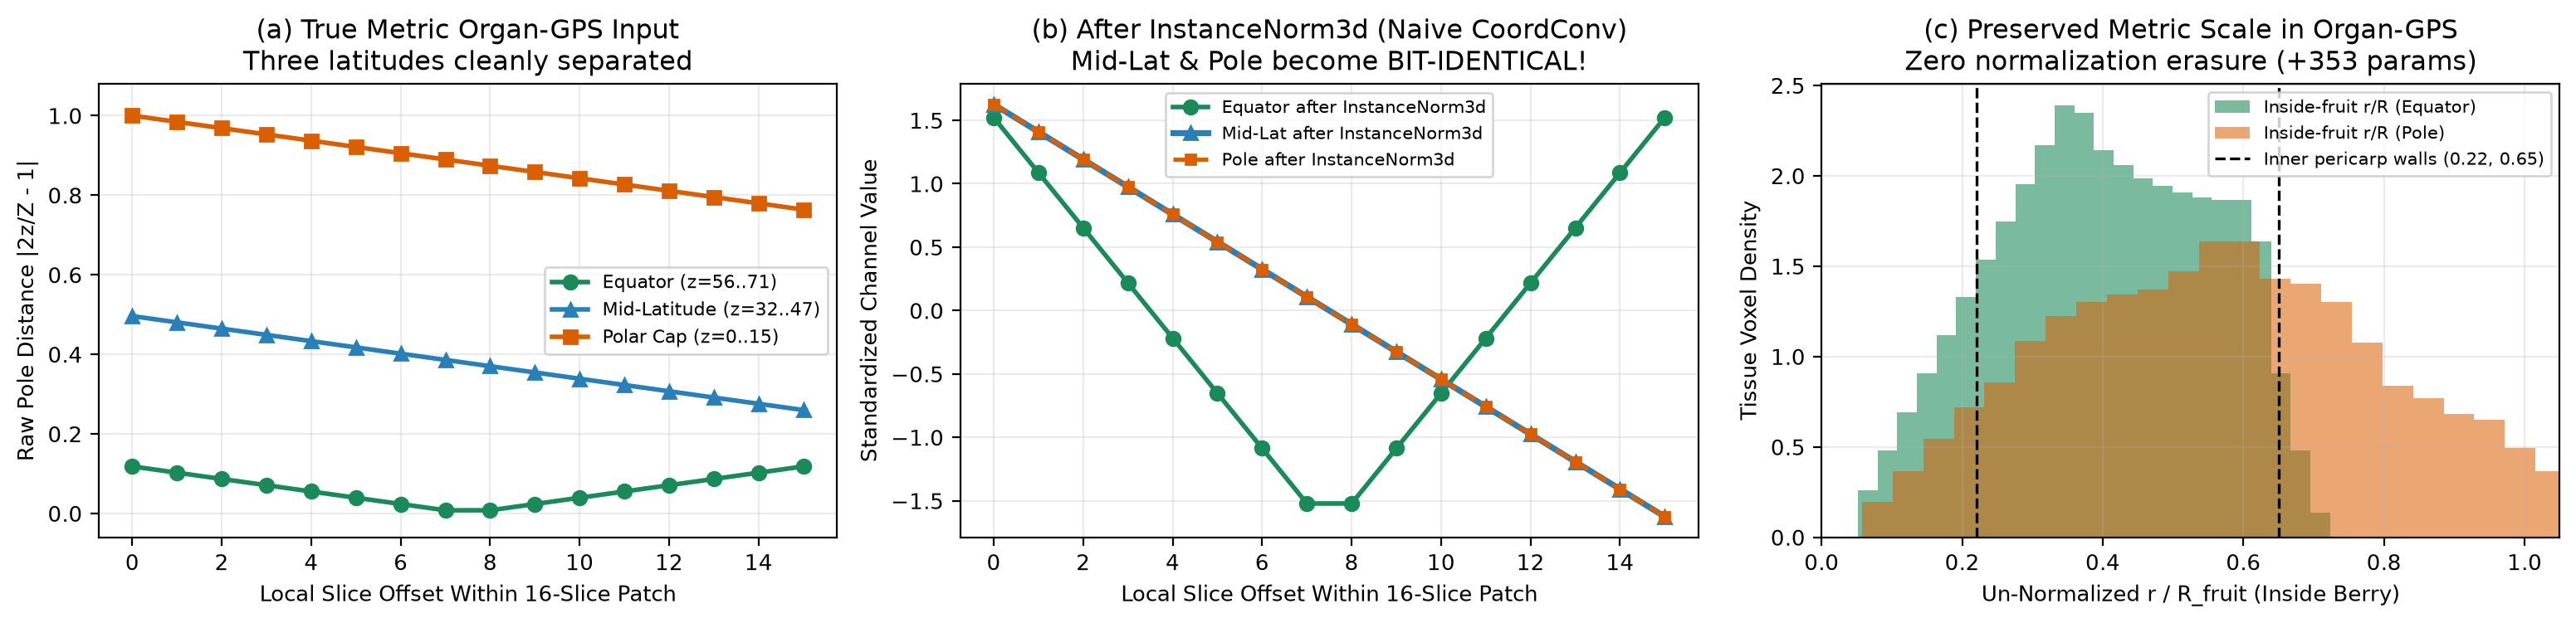
\includegraphics[width=\textwidth]{../figures/fig03_instancenorm_coordinate_erasure.png}
    \vspace{-4pt}
    \caption*{\footnotesize\textit{Executed Figure~3 (\texttt{Out [2]}, saved as \texttt{fig03\_instancenorm\_coordinate\_erasure.png}): (a)~Raw metric pole distance $|2z/Z - 1|$ cleanly separating Equator, Mid-Latitude, and Polar Cap; (b)~after patch-wise \texttt{InstanceNorm3d}, Mid-Latitude and Polar Cap collapse to bit-identical profiles ($\max|\Delta| = 4.77 \times 10^{-7}$); (c)~preserved un-normalized radial metric scale in \texttt{Organ-GPS} ($+353$ params).}}
\end{figure}

\section*{2. Comparing Fuzzy Implication Families \& LTN $p$-Mean Gradient Amplification}
\addcontentsline{toc}{section}{\texorpdfstring{2. Comparing Fuzzy Implication Families \& LTN $p$-Mean Gradient Amplification}{2. Comparing Fuzzy Implication Families and LTN p-Mean Gradient Amplification}}

\begin{guidehdr}
{\small\bfseries\color{kiwigreen!75!black}Conceptual \& Mathematical Guide: Differentiable Fuzzy Implications \& LTN $p$-Mean Hard-Counterexample Mining}
\end{guidehdr}

\subsubsection*{2.1 Part A --- Turning Biological Rules into Smooth Gradients (Fuzzy Implications \& $T$-Norms)}
Why can we not drop classical Boolean \texttt{if /\allowbreak{} else} rules directly into PyTorch training? Because discrete truth values $\{0, 1\}$ behave like step functions: their derivative is $0$ almost everywhere and undefined at the jump, giving backpropagation no usable direction to adjust neural weights.

\textbf{Logic Tensor Networks (LTN)} ground first-order logic in \textbf{Real Logic} over the continuous interval $[0, 1]$. For every unlabeled voxel $\mathbf{x} \in \Omega_U$, we encode the botanical exclusion law:
\[
\forall \mathbf{x} \in \Omega_U:\quad \underbrace{\neg R_{\text{ring}}(\mathbf{x})}_{\text{premise } a \;=\; 1 - R_{\text{ring}}(\mathbf{x})} \;\Longrightarrow\; \underbrace{\neg \text{Seed}(\mathbf{x})}_{\text{conclusion } b \;=\; 1 - p_\theta(\mathbf{x})}
\]
(\textit{``If voxel $\mathbf{x}$ lies outside the valid inner-pericarp ring, then the network must NOT predict a seed there.''})

A \textbf{fuzzy implication} $I(a, b) \in [0, 1]$ measures how strongly $a \Rightarrow b$ holds; its \textbf{violation (penalty)} is $v(a, b) = 1 - I(a, b) \in [0, 1]$. Comparing the three canonical fuzzy-logic families (\texttt{kns.implication\_violation}) on $(a = 1 - R_{\text{ring}},\, b = 1 - p_\theta)$ explains why only \textbf{Product (Reichenbach)} logic is well-suited to deep learning:

\vspace{0.3em}
{\footnotesize
\setlength{\tabcolsep}{4pt}
\renewcommand{\arraystretch}{1.24}
\rowcolors{2}{rowalt}{white}
\begin{tabularx}{\textwidth}{L{2.75cm} L{2.25cm} L{2.45cm} L{3.05cm} Y}
\toprule
\rowcolor{uibblue!12}\textbf{Fuzzy Logic Family} & \textbf{$T$-Norm $T(a, b)$} & \textbf{Implication $I(a, b)$} & \textbf{Violation $v = 1 - I$ on $(\neg R_{\text{ring}} \Rightarrow \neg p_\theta)$} & \textbf{Gradient $\partial v / \partial p_\theta$ \& Optimization Behavior} \\
\midrule
\textbf{Product (Reichenbach)} & $a \cdot b$ & $1 - a(1 - b)$ & $p_\theta\,(1 - R_{\text{ring}})$ & $1 - R_{\text{ring}} > 0$ \textbf{everywhere for $R_{\text{ring}} < 1$} --- smooth, bilinear, obeys contraposition ($\text{Seed} \Rightarrow R_{\text{ring}}$ yields the exact same $v$), \textbf{zero dead zones}. \\
\textbf{\L{}ukasiewicz} & $\max(0,\, a + b - 1)$ & $\min(1,\, 1 - a + b)$ & $\max(0,\, p_\theta - R_{\text{ring}})$ & $1$ if $p_\theta > R_{\text{ring}}$, else \textbf{$0$} --- creates a large \textbf{zero-gradient dead triangle} whenever $p_\theta \le R_{\text{ring}}$ (e.g., an FP with $p_\theta = 0.35$ in a soft transition zone $R_{\text{ring}} = 0.40$ receives zero gradient!). \\
\textbf{G\"odel (Minimum)} & $\min(a, b)$ & $1$ if $a \le b$ else $b$ & $0$ if $p_\theta \le R_{\text{ring}}$ else $p_\theta$ \textit{(or $1 - R_{\text{ring}}$ under $\text{Seed} \Rightarrow R_{\text{ring}}$)} & \textbf{Discontinuous jump} along $p_\theta = R_{\text{ring}}$, breaks contraposition, keeps the dead triangle, and has $\partial v / \partial p_\theta = 0$ almost everywhere under $\text{Seed} \Rightarrow R_{\text{ring}}$ --- unsuitable for smooth SGD. \\
\bottomrule
\end{tabularx}
}
\vspace{0.3em}

Because G\"odel logic is discontinuous and untrainable in standard form, the code plots the two continuous landscapes side-by-side in \textbf{Figure 4a (Product)} and \textbf{Figure 4b (\L{}ukasiewicz)}.

\subsubsection*{2.2 Part B --- Universal Quantification ($\forall \mathbf{x}$) via LTN's Generalized $p$-Mean}
A universal axiom must hold for \textbf{all} voxels in an unlabeled 3D patch. Consider a realistic $64 \times 40 \times 16$ polar-cap cube containing $N = 40{,}960$ voxels, where \textbf{$99.2\%$} ($n_{\text{BG}} = 40{,}632$ voxels) are quiet background ($v_{\text{BG}} = 0.01$) and only \textbf{$0.8\%$} ($n_{\text{FP}} = 328$ voxels) are severe vascular false positives ($v_{\text{FP}} = 0.95$). If we simply take the arithmetic mean ($p = 1$), the $99.2\%$ compliant background voxels dilute the rare $0.8\%$ violations.

LTN solves this dilution using the \textbf{generalized $p$-mean universal error aggregator} (\texttt{kns.ltn\_universal\_pmean}, with $p \ge 1$ and $\varepsilon = 10^{-8}$ ensuring numerical smoothness at $v_i = 0$):
\[
\mathcal{L}_p(\mathbf{v}) = 1 - \operatorname{Agg}_{\forall, p}(1 - \mathbf{v}) = \left(\frac{1}{N}\sum_{i=1}^{N} v_i^{p} + \varepsilon\right)^{1/p}.
\]

\textbf{Exact Gradient Derivation (Chain Rule):} Neglecting $\varepsilon \ll \frac{1}{N}\sum_j v_j^p$, differentiating $\mathcal{L}_p$ with respect to each voxel's violation $v_i$ gives:
\[
\frac{\partial \mathcal{L}_p}{\partial v_i} = \frac{1}{p}\left(\frac{1}{N}\sum_{j=1}^{N} v_j^p\right)^{\frac{1}{p} - 1} \cdot \frac{p}{N}\,v_i^{p-1} = \frac{1}{N}\left(\frac{v_i}{\mathcal{L}_p}\right)^{p-1}.
\]

Three crucial consequences follow directly from this derivative:
\begin{enumerate}
\item \textbf{Automatic hard-counterexample focusing (\texttt{fp\_bg\_ratio} \& \texttt{pct\_grad\_on\_fp}):} Taking the ratio of gradients between a violating FP voxel and a clean background voxel cancels $N$ and $\mathcal{L}_p$:
\[
\frac{\partial \mathcal{L}_p / \partial v_{\text{FP}}}{\partial \mathcal{L}_p / \partial v_{\text{BG}}} = \left(\frac{v_{\text{FP}}}{v_{\text{BG}}}\right)^{p-1} = 95^{\,p-1} \quad\Longrightarrow\quad \frac{G_{\text{FP}}}{G_{\text{BG}}} = \frac{n_{\text{FP}}}{n_{\text{BG}}}\left(\frac{v_{\text{FP}}}{v_{\text{BG}}}\right)^{p-1}.
\]
At $p = 1$ (plain mean), $95^0 = 1$: every voxel gets equal weight, leaving just \textbf{\texttt{0.80\%}} of the gradient on the actual FPs (\texttt{fp\_bg\_ratio} $\approx 0.008$). At \textbf{$p = 3$}, each FP voxel receives $95^2 = \mathbf{9{,}025\times}$ stronger per-voxel gradient than background, flipping \texttt{fp\_bg\_ratio} to \textbf{\texttt{72.85}} and channeling \textbf{\texttt{98.65\%}} of the entire optimization step onto the \texttt{0.8\%} violations!
\item \textbf{Absolute FP gradient amplification (\texttt{grad\_fp} \& \texttt{gain\_vs\_p1}):} Summing over all $n_{\text{FP}}$ violating voxels yields $G_{\text{FP}}(p) = \frac{n_{\text{FP}}}{N}\left(v_{\text{FP}} / \mathcal{L}_p\right)^{p-1}$. Compared to plain averaging ($G_{\text{FP}}(1) = 0.0080$), the absolute FP gradient grows by $\left(v_{\text{FP}} / \mathcal{L}_p\right)^{p-1}$---an amplification of \textbf{$\approx 24.98\times$} at $p = 3$ ($\mathcal{L}_3 \approx 0.1901$).
\item \textbf{Why $p \in \{2, 3\}$ is the sweet spot (and not $p \ge 6$):} As $p \to \infty$, $\mathcal{L}_p(\mathbf{v}) \to \max_i v_i$, collapsing the entire update onto whichever single noisy voxel happens to be largest and causing high-variance SGD steps. Setting $p = 3$ achieves smooth, stable hard-counterexample mining.
\end{enumerate}

\subsubsection*{2.3 What the Code Below Computes (Table 2 \& Figure 4)}
\begin{enumerate}
\item Evaluates \texttt{V\_prod} and \texttt{V\_luka} across a $120 \times 120$ mesh of $(R_{\text{ring}},\, p_\theta) \in [0, 1]^2$.
\item Sweeps $p \in \{1.0, 1.5, 2.0, 3.0, 4.0, 6.0, 8.0\}$ on the simulated $40{,}960$-voxel polar cube using PyTorch autograd (\texttt{v.requires\_grad\_(True)} and \texttt{lv.backward()}) to confirm our analytical gradient laws numerically.
\item Displays \textbf{Table 2} (\texttt{df\_p}), exports all Section 1--2 quantitative metrics to \texttt{../\allowbreak{}results/\allowbreak{}nb02\_instancenorm\_and\_ltn.json}, and generates the 4-panel \textbf{Figure 4} (\texttt{(a)} Product vs. \texttt{(b)} \L{}ukasiewicz violation contours; \texttt{(c)} loss severity $\mathcal{L}_p$; \texttt{(d)} FP gradient gain vs. $p = 1$).
\end{enumerate}

\begin{codebox}[{In [3] $\cdot$ Python --- Fuzzy implication surfaces \& LTN $p$-mean autograd gradient-amplification sweep}]
\begin{lstlisting}[style=pybmed]
# Compare Product (Reichenbach), Łukasiewicz, and Gödel violation surfaces on premise = (1 - R_ring), conclusion = (1 - p_theta)
r_vals = np.linspace(0.0, 1.0, 120)
p_vals = np.linspace(0.0, 1.0, 120)
RR, PP = np.meshgrid(r_vals, p_vals)
prem_t = torch.from_numpy((1.0 - RR).astype(np.float32))
conc_t = torch.from_numpy((1.0 - PP).astype(np.float32))
V_prod = kns.implication_violation(prem_t, conc_t, "product").numpy()
V_luka = kns.implication_violation(prem_t, conc_t, "lukasiewicz").numpy()

# Quantifier power sweep on simulated 64 x 40 x 16 = 40,960-voxel polar cube with 0.8% (328 voxels) vascular FPs
n_vox = 64 * 40 * 16
n_fp = int(round(0.008 * n_vox))
p_grid = [1.0, 1.5, 2.0, 3.0, 4.0, 6.0, 8.0]
p_rows = []
g0 = None
for pv in p_grid:
    v = torch.full((n_vox,), 0.01, dtype=torch.float32)
    v[:n_fp] = 0.95
    v.requires_grad_(True)
    lv = kns.ltn_universal_pmean(v, p=pv)
    lv.backward()
    g_fp = float(v.grad[:n_fp].sum().item())
    g_bg = float(v.grad[n_fp:].sum().item())
    if g0 is None:
        g0 = g_fp
    p_rows.append({
        "p": pv,
        "loss": round(float(lv.item()), 4),
        "grad_fp": round(g_fp, 4),
        "fp_bg_ratio": g_fp / max(g_bg, 1e-12),
        "gain_vs_p1": round(g_fp / g0, 2),
        "pct_grad_on_fp": round(100.0 * g_fp / (g_fp + g_bg), 2),
    })

df_p = pd.DataFrame(p_rows)
display(df_p)

out_nb02 = {
    "raw_means": {"equator": round(float(z_eq_r.mean()), 4), "mid_lat": round(float(z_mid_r.mean()), 4), "pole": round(float(z_pol_r.mean()), 4)},
    "inorm_means": {"equator": round(float(z_eq_i.mean()), 6), "mid_lat": round(float(z_mid_i.mean()), 6), "pole": round(float(z_pol_i.mean()), 6)},
    "max_diff_mid_pol_after_inorm": max_diff_mid_pol_after,
    "param_counts": {"baseline": n_base, "additive_gps": n_add, "coupled_gps": n_cpl},
    "pmean_sweep": p_rows,
}
(RES_DIR / "nb02_instancenorm_and_ltn.json").write_text(json.dumps(out_nb02, indent=2), encoding="utf-8")

# Figure 4: 4-Panel Fuzzy Implications & LTN p-Mean Gradient Dynamics
fig, axes = plt.subplots(1, 4, figsize=(17.0, 3.8))

im0 = axes[0].contourf(RR, PP, V_prod, levels=16, cmap="inferno")
axes[0].set_xlabel("R_ring(x)")
axes[0].set_ylabel("Neural Seed Prob p_theta(x)")
axes[0].set_title("(a) Product (Reichenbach) T-Norm\nSmooth gradients everywhere!")
plt.colorbar(im0, ax=axes[0], fraction=0.046, pad=0.03)

im1 = axes[1].contourf(RR, PP, V_luka, levels=16, cmap="inferno")
axes[1].set_xlabel("R_ring(x)")
axes[1].set_ylabel("Neural Seed Prob p_theta(x)")
axes[1].set_title("(b) Łukasiewicz Implication\nZero-gradient dead triangle (black)!")
plt.colorbar(im1, ax=axes[1], fraction=0.046, pad=0.03)

axes[2].plot(df_p["p"], df_p["loss"], "o-", color="#2c3e50", lw=2.1)
axes[2].axvline(3.0, color="#1b8a5a", ls="--", lw=1.6, label="Chosen LTN p = 3")
axes[2].set_xlabel("Quantifier Exponent p")
axes[2].set_ylabel("Aggregate Loss L_p")
axes[2].set_title("(c) Loss Severity on 0.8% Polar FPs\np=1: 0.0175 -> p=3: 0.1901")
axes[2].legend(fontsize=7.6)
axes[2].grid(alpha=0.25)

axes[3].plot(df_p["p"], df_p["gain_vs_p1"], "s-", color="#e67e22", lw=2.1)
axes[3].axvline(3.0, color="#1b8a5a", ls="--", lw=1.6, label="p = 3 (25.0× gain, 98.6% on FPs)")
axes[3].set_xlabel("Quantifier Exponent p")
axes[3].set_ylabel("FP Gradient Gain vs. p = 1")
axes[3].set_title("(d) Hard-Counterexample Mining\nAmplifies rare OOD gradients >25×")
axes[3].legend(fontsize=7.4)
axes[3].grid(alpha=0.25)

plt.tight_layout()
fig.savefig(FIG_DIR / "fig04_tnorms_and_pmean_gradients.png", bbox_inches="tight")
plt.show()
\end{lstlisting}
\end{codebox}
\begin{outbox}[{Out [3] $\cdot$ DataFrame --- LTN Generalized $p$-Mean Quantifier Sweep ($40{,}960$-voxel polar cube, $0.8\%$ FPs; saved to \texttt{nb02\_instancenorm\_and\_ltn.json})}]
\centering
{\scriptsize
\setlength{\tabcolsep}{3.6pt}
\renewcommand{\arraystretch}{1.18}
\rowcolors{2}{rowalt}{white}
\begin{tabular}{r r r r r r}
\toprule
\rowcolor{uibblue!12}\textbf{p} & \textbf{loss} & \textbf{grad\_fp} & \textbf{fp\_bg\_ratio} & \textbf{gain\_vs\_p1} & \textbf{pct\_grad\_on\_fp} \\
\midrule
1.0 & 0.0175 & 0.0080 & 8.072455e-03 & 1.00 & 0.80 \\
1.5 & 0.0413 & 0.0384 & 7.868055e-02 & 4.79 & 7.29 \\
2.0 & 0.0856 & 0.0889 & 7.668831e-01 & 11.10 & 43.40 \\
\textbf{3.0} & \textbf{0.1901} & \textbf{0.2000} & \textbf{7.285391e+01} & \textbf{24.98} & \textbf{98.65} \\
4.0 & 0.2842 & 0.2991 & 6.921120e+03 & 37.36 & 99.99 \\
6.0 & 0.4249 & 0.4473 & 6.246313e+07 & 55.86 & 100.00 \\
8.0 & 0.5196 & 0.5469 & 5.469387e+11 & 68.30 & 100.00 \\
\bottomrule
\end{tabular}
}
\end{outbox}
\begin{figure}[H]
    \centering
    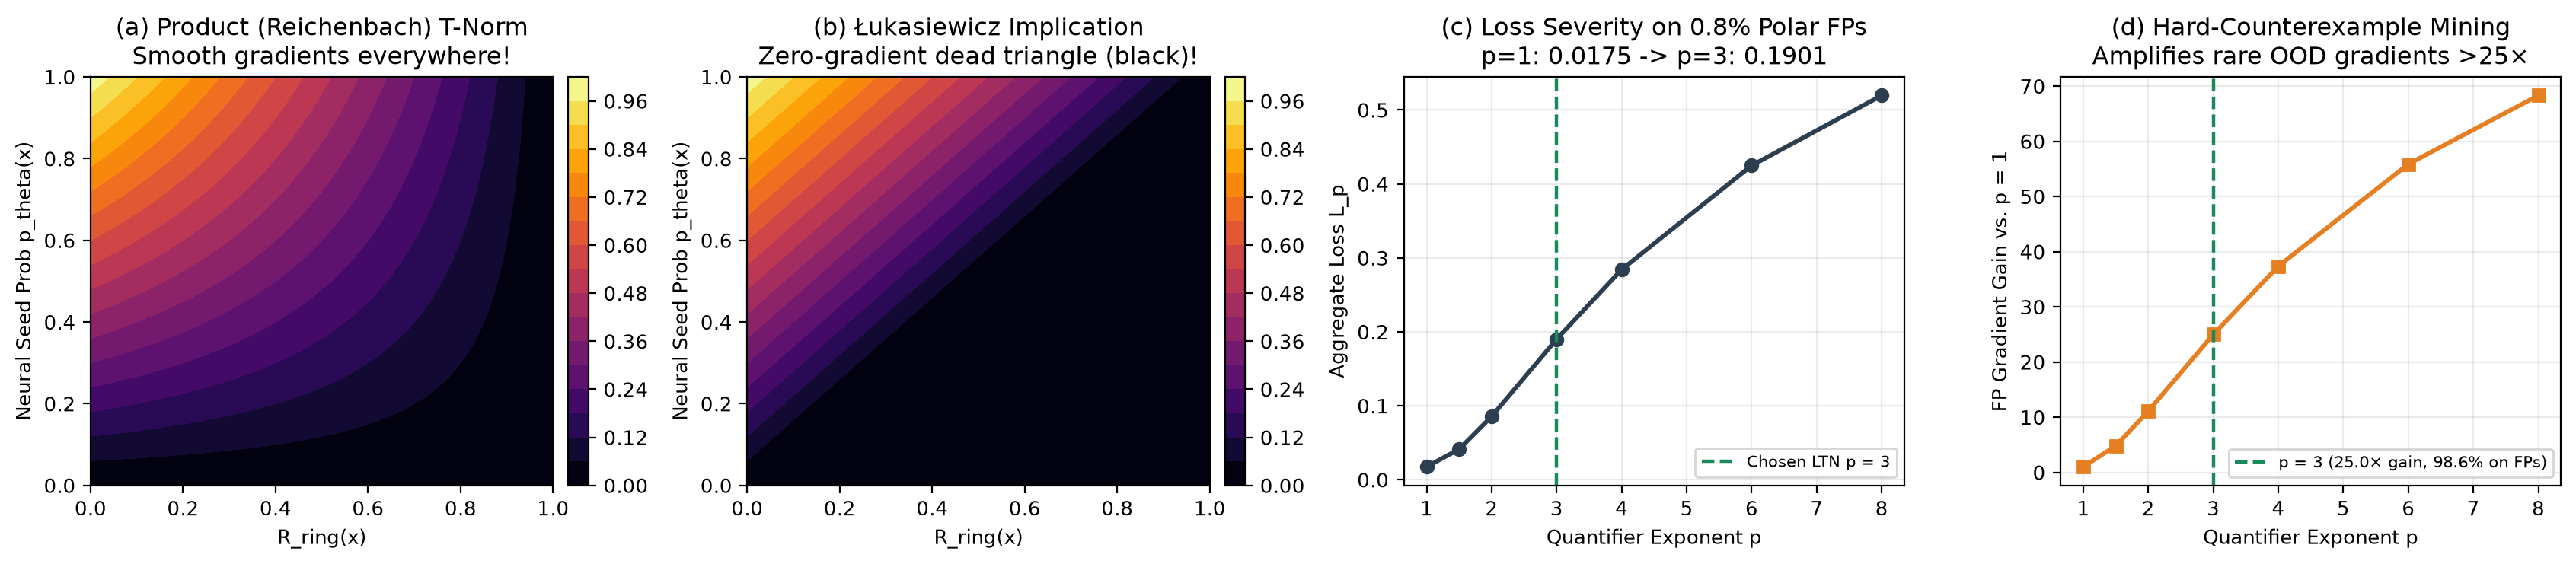
\includegraphics[width=\textwidth]{../figures/fig04_tnorms_and_pmean_gradients.png}
    \vspace{-4pt}
    \caption*{\footnotesize\textit{Executed Figure~4 (\texttt{Out [3]}, saved as \texttt{fig04\_tnorms\_and\_pmean\_gradients.png}): (a)~Smooth Reichenbach Product violation surface vs.\ (b)~\L{}ukasiewicz zero-gradient dead triangle; (c)~aggregate universal loss $\mathcal{L}_p$ and (d)~rare-FP gradient amplification across $p \in [1, 8]$ ($24.98\times$ gain and $98.65\%$ gradient focus on $0.8\%$ polar FPs at $p = 3$).}}
\end{figure}

\end{document}
